% -*- latex -*-
%%%%%%%%%%%%%%%%%%%%%%%%%%%%%%%%%%%%%%%%%%%%%%%%%%%%%%%%%%%%%%%%
%%%%%%%%%%%%%%%%%%%%%%%%%%%%%%%%%%%%%%%%%%%%%%%%%%%%%%%%%%%%%%%%
%%%%
%%%% This text file is part of the source of 
%%%% `Parallel Programming in MPI and OpenMP'
%%%% by Victor Eijkhout, copyright 2012-2020
%%%%
%%%% tau.tex : tutorial about tracing with TAU
%%%%
%%%%%%%%%%%%%%%%%%%%%%%%%%%%%%%%%%%%%%%%%%%%%%%%%%%%%%%%%%%%%%%%
%%%%%%%%%%%%%%%%%%%%%%%%%%%%%%%%%%%%%%%%%%%%%%%%%%%%%%%%%%%%%%%%

\Level 0 {Timing}

Many systems have their own timers:
\begin{itemize}
\item MPI see section~\ref{sec:mpi-timing};
\item OpenMP see section~\ref{sec:omp-timing};
\item PETSc see section~\ref{sec:petsc-timing}.
\end{itemize}

\Level 1 {Parallel timing}

Timing parallel operations is fraught with peril,
as processes or threads can interact with each other.
This means that you may be measuring the wait time
induced by synchronization.
Sometimes that is actually what you want,
as in the case of a \indexterm{ping-pong} operation;
section~\ref{sec:mpi-send-recv}.

Other times, this is not what you want.
Consider the code
\begin{lstlisting}
if (procno==0)
  do_big_setup();
t = timer();
mpi_some_collective();
duration = timer() - t;
\end{lstlisting}

\begin{figure}[ht]
  \hbox\bgroup
  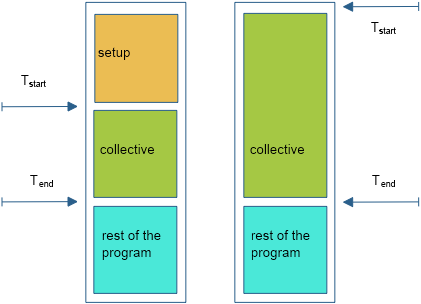
\includegraphics[scale=.5]{timenobarrier}
  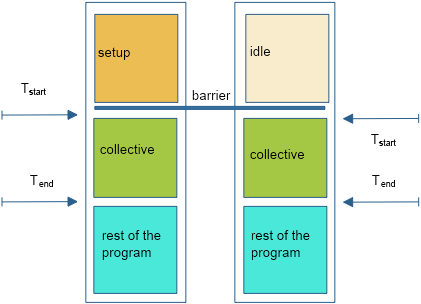
\includegraphics[scale=.5]{timebarrier}
  \egroup
  \caption{Timing a parallel code without and with barrier}
  \label{fig:time-collective}
\end{figure}

Figure~\ref{fig:time-collective} illustrates this:
\begin{itemize}
\item in the naive scenario, processes other than zero start the collective immediately,
  but process zero first does the setup;
\item all processes presumably finish more or less together.
\end{itemize}
On the non-zero processes we now get a time measurement,
which we intended to be just the collective operation,
that includes the setup time of process zero.

The solution is to put a barrier around the section that you want to time;
see again figure~\ref{fig:time-collective}.

\input tutorials/tau
